\section{Closing Thoughts}

\begin{frame}{Next Steps}
\begin{columns}
\begin{column}{0.6\textwidth}
\begin{itemize}
\item investigate structural changes in gene regulatory networks induced by plasticity
\item investigate interaction of direct and indirect plasticity
\item attempt to demonstrate situation where search with plasticity outperforms search without
\end{itemize}
\end{column}
\begin{column}{0.4\textwidth}
\begin{center}
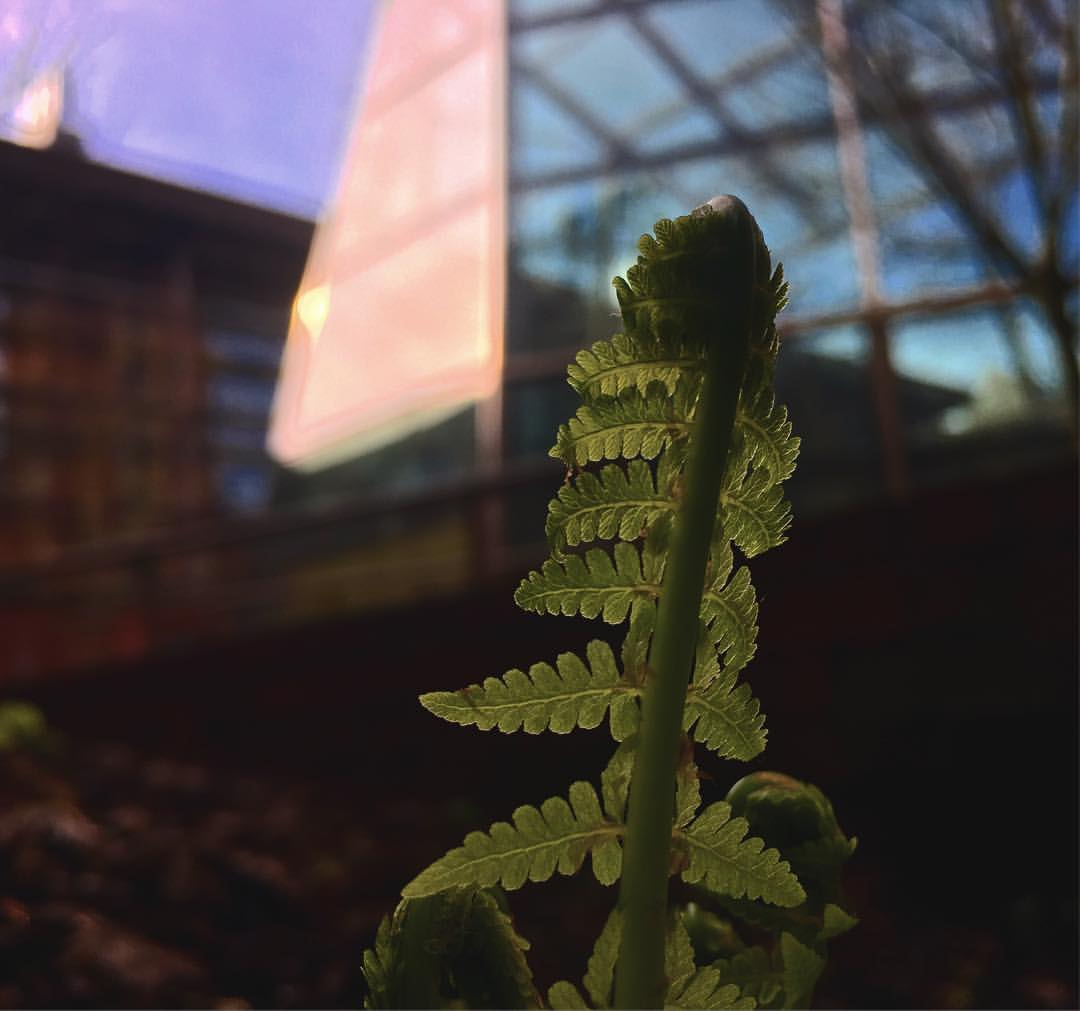
\includegraphics[width=\textwidth,trim={7cm 0 8cm 0},clip]{img/oppfern}
\end{center}
\end{column}
\end{columns}
\end{frame}

\begin{frame}{Closing Thoughts: Practical Applications}
\begin{figure}
  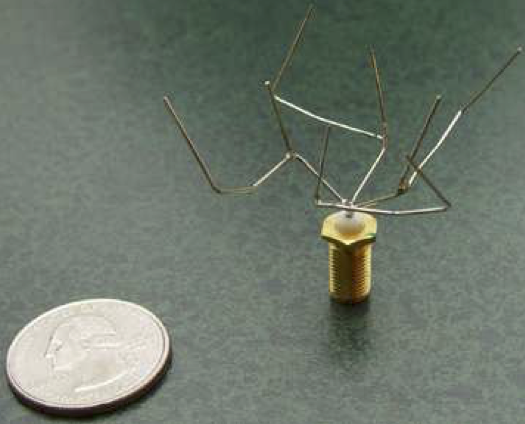
\includegraphics[width=0.7\textwidth]{img/evolved_antenna} 
  \hspace{2ex}
  \caption{A spacecraft antenna design generated using evolutionary methods \cite[Figure 2(a)]{Hornby2006AutomatedAlgorithms}.}
  \label{fig:evolved_antenna}
\end{figure}
\end{frame}

\begin{frame}{Closign Thoughts: Scientific Questions}
\begin{columns}
\begin{column}{0.6\textwidth}
\begin{itemize}
\item at what level of abstraction can the power of biological evolution be harnessed in a computational model?
\item what are the fundamental mechanisms at play in evolution?
\end{itemize}
\end{column}
\begin{column}{0.4\textwidth}
\begin{center}
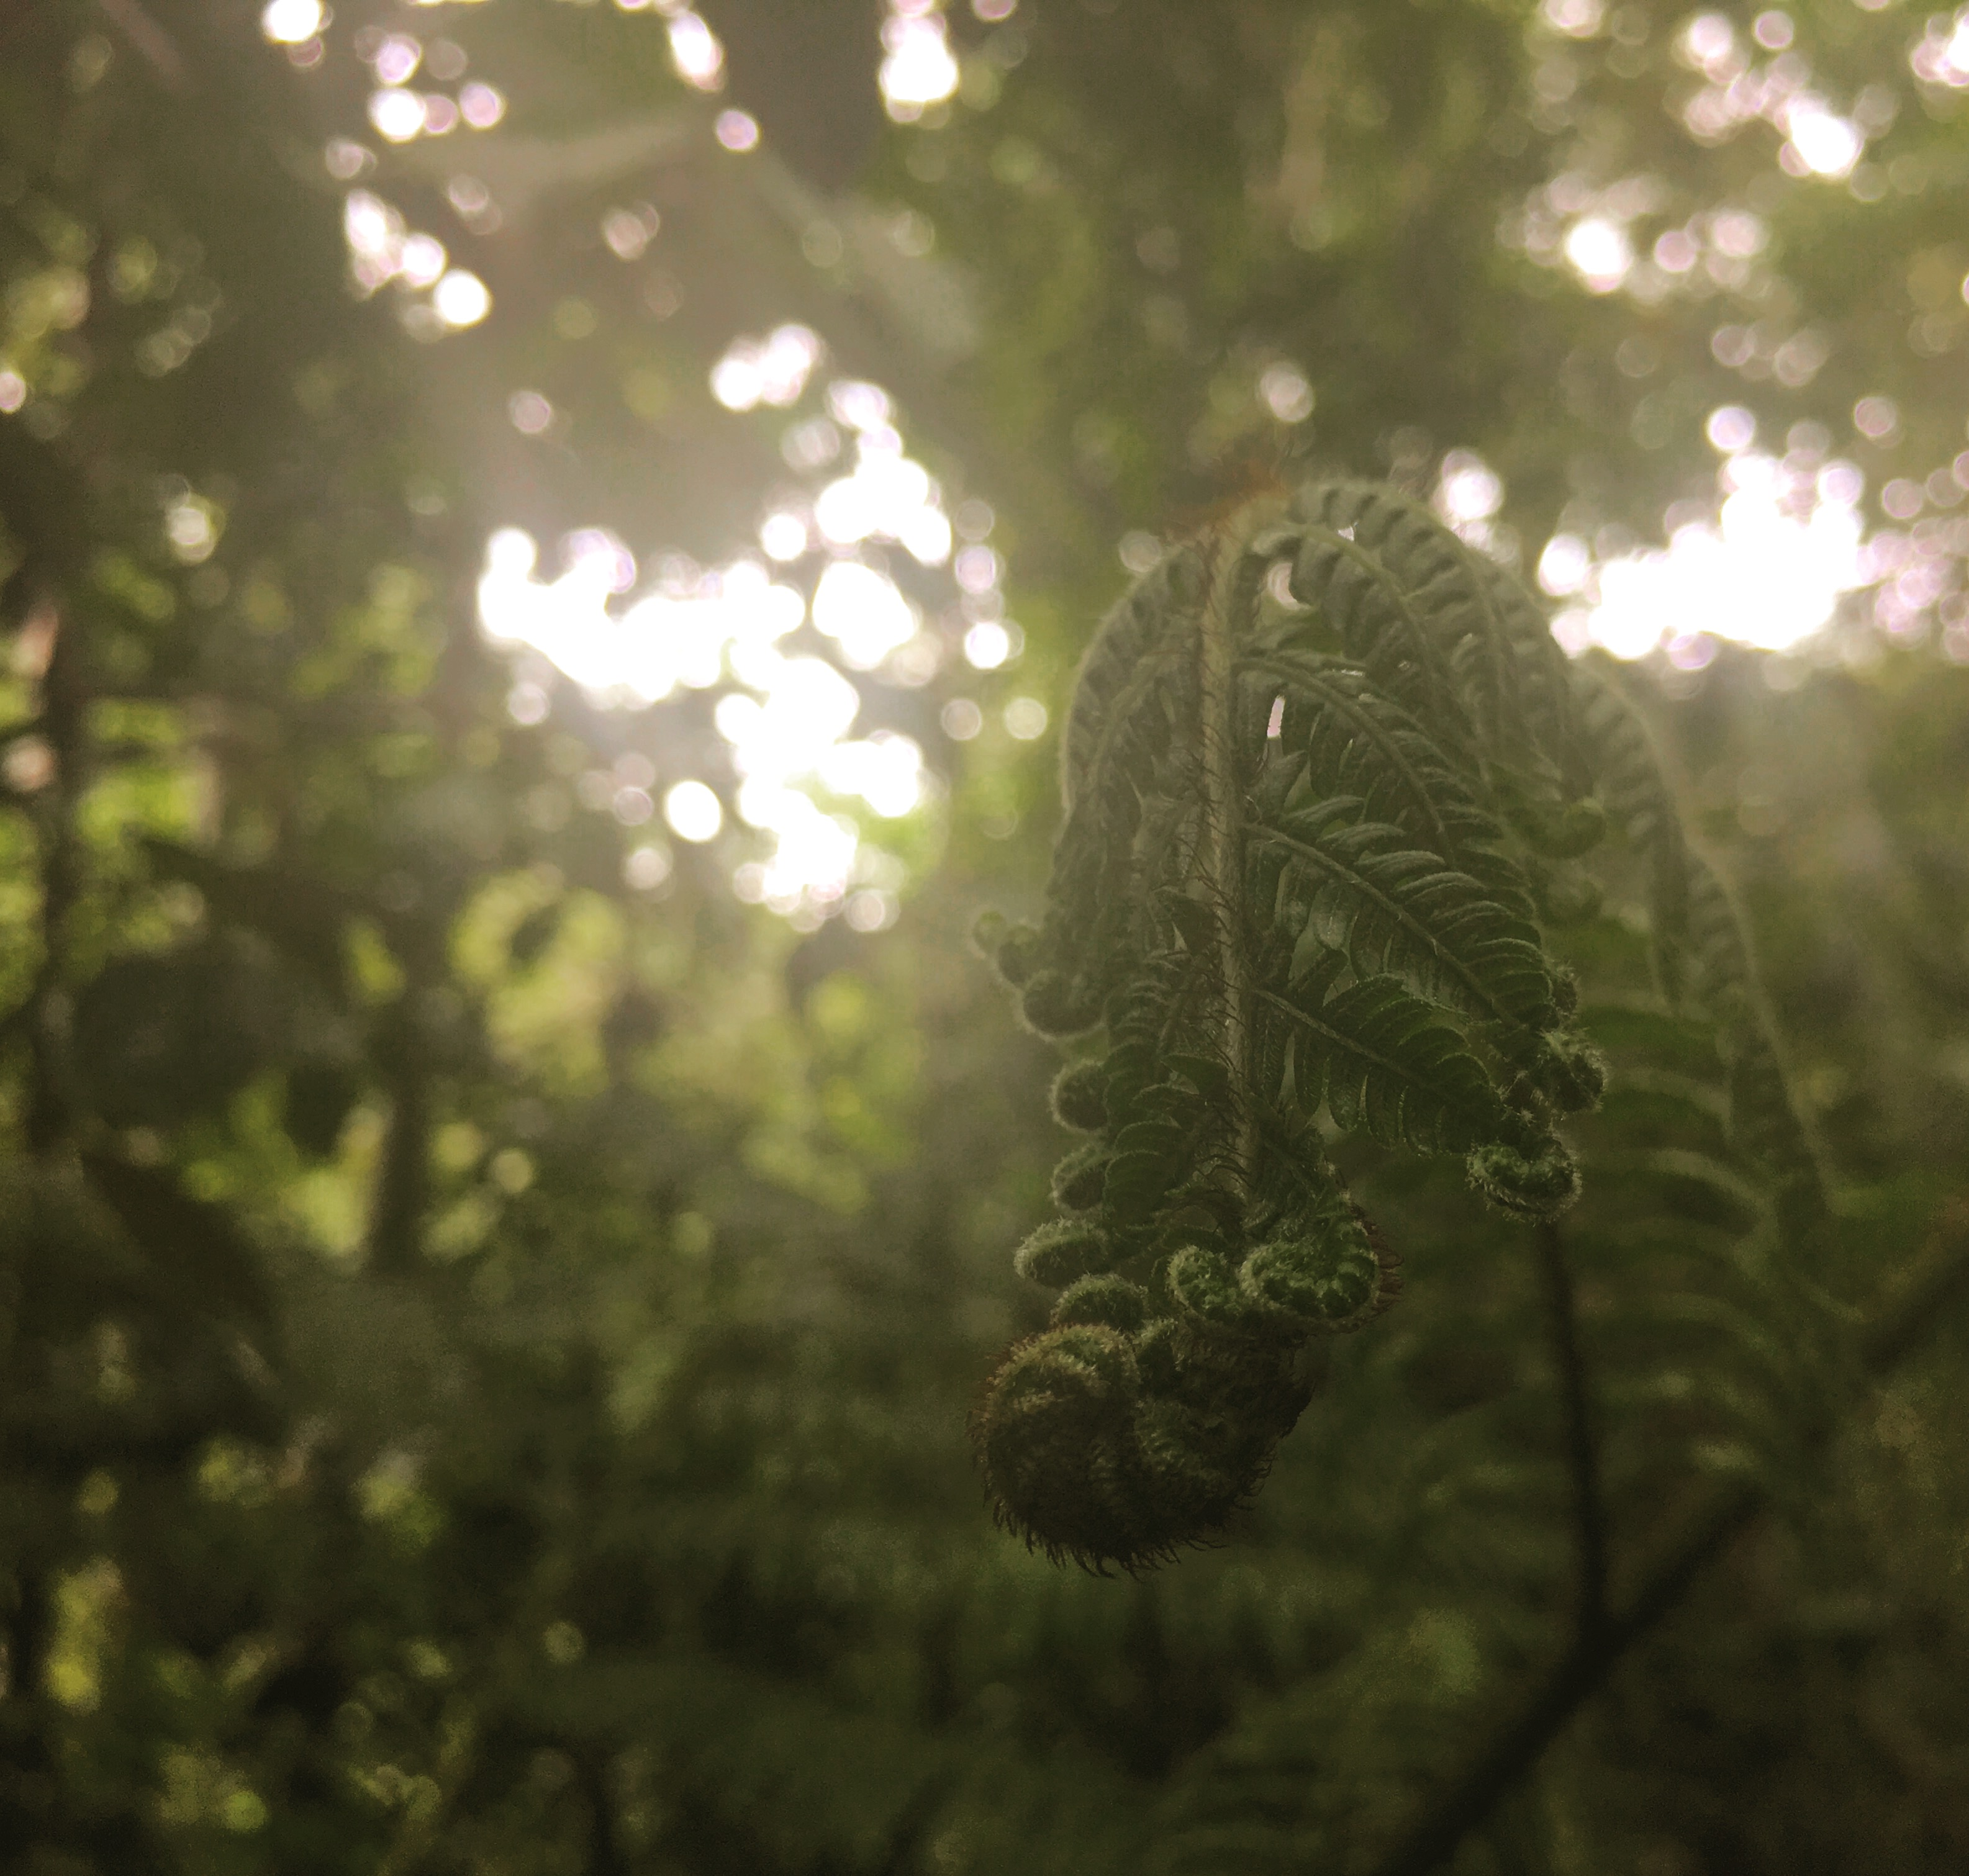
\includegraphics[width=\textwidth,trim={18cm 0 27cm 0},clip]{img/tropical_fern}
\end{center}
\end{column}
\end{columns}
\end{frame}

\begin{frame}{Closing Thoughts: Scientific Questions}
\begin{columns}
\begin{column}{0.6\textwidth}
\begin{itemize}
\item evolutionary biology provides continuing inspiration for new techniques in evolutionary computing
\item evolutionary models move theory evaluation from a qualitative endeavor towards a quantitative endeavor
\end{itemize}
\end{column}
\begin{column}{0.4\textwidth}
\begin{center}
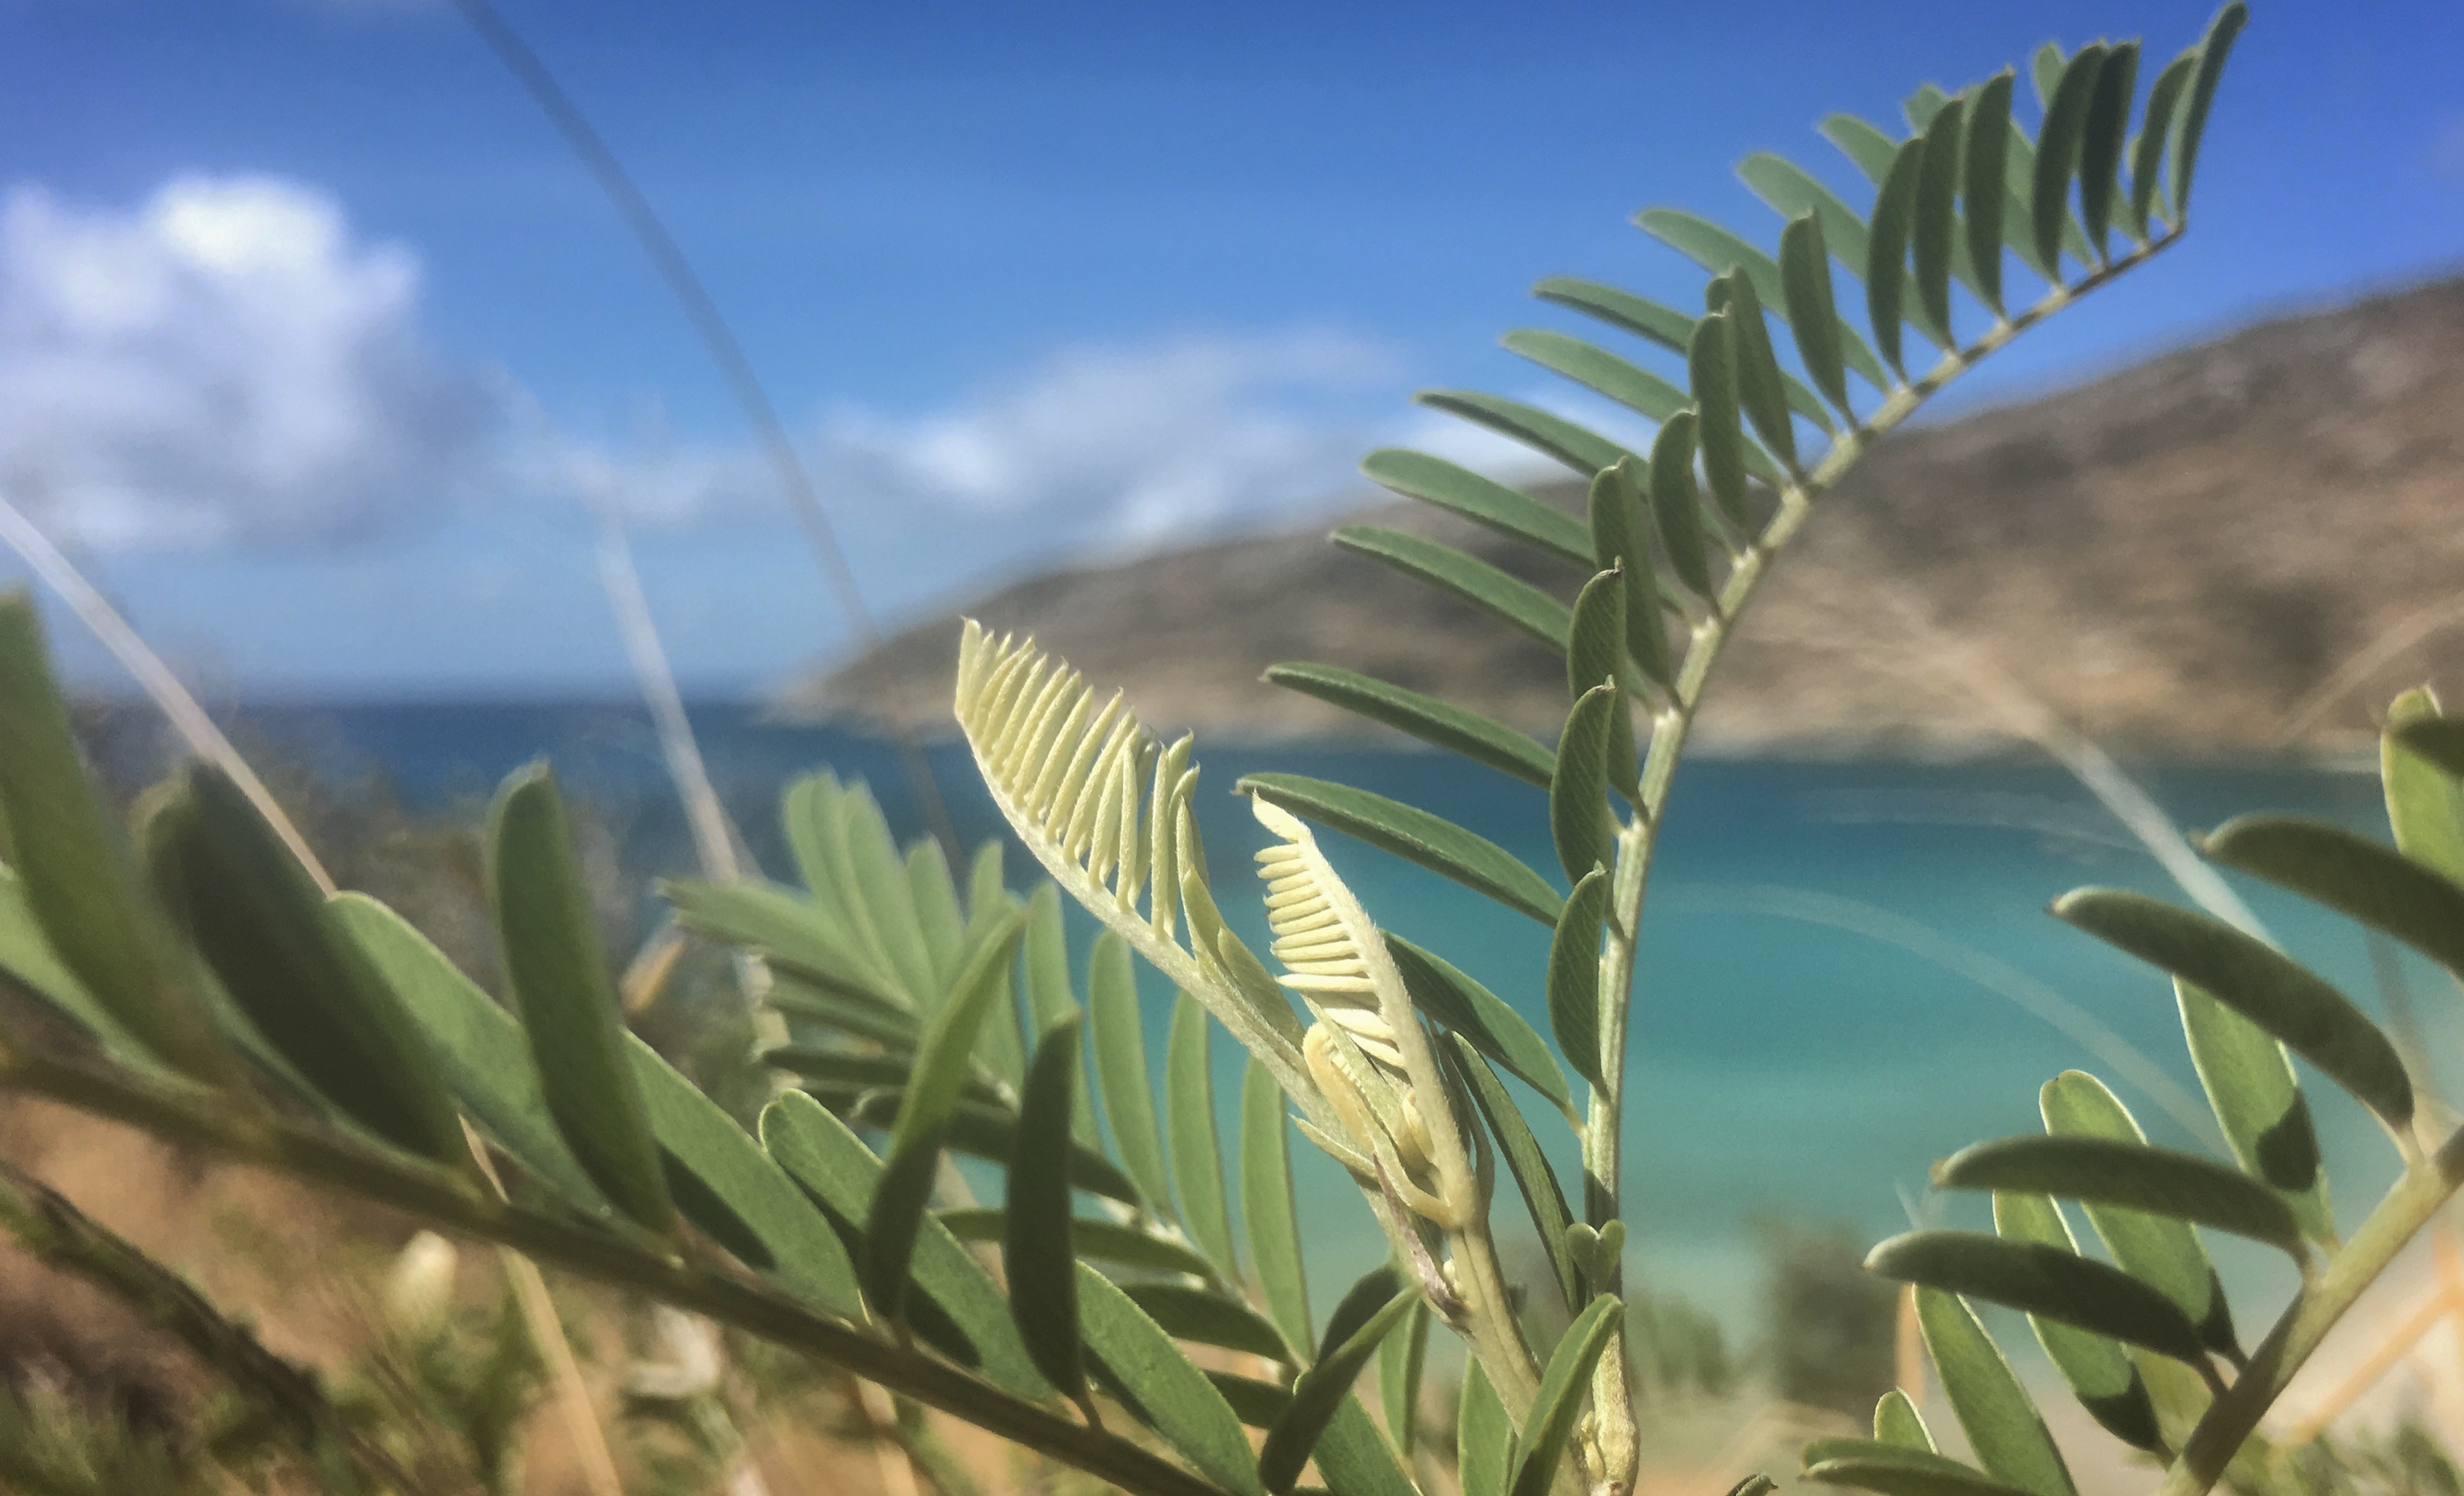
\includegraphics[width=\textwidth,trim={43cm 0 47cm 0},clip]{img/island_fern}
\end{center}
\end{column}
\end{columns}
\end{frame}

% \begin{frame}{Scientific Questions}
% \begin{displayquote}
% ``Many evolutionary biologists do not see a need to connect somatic adaptability to the generation of variation, and some see a need to keep them separate. For them, it is sufficient to say that random mutation is required and that the phenotypic variation arises haphazardly from it as random damage; the organism's current phenotype does not matter for the variation produced, and the output of variation is nearly random \cite[p 219]{Kirschner2005TheDilemma}.''
% \end{displayquote}
% \end{frame}